\documentclass[conference]{IEEEtran}

\usepackage{amsmath,amssymb}
\usepackage{graphicx}
\usepackage{booktabs}
\usepackage{array}
\usepackage{url}
\usepackage{cite}
\usepackage{textcomp}

\setlength{\emergencystretch}{2em}
\hyphenation{Coin-Gecko Fire-base Spring-Boot Tensor-Flow}

\begin{document}

\title{AI Crypto Predictor: A Native Android System for Cryptocurrency Market Monitoring and Uncertainty-Aware Price-Direction Prediction}

\author{
\IEEEauthorblockN{Kevin Doss\IEEEauthorrefmark{1}, Shreyas Kamble\IEEEauthorrefmark{2}, Samarth Kale\IEEEauthorrefmark{3}, Rakhi Kalantri\IEEEauthorrefmark{4}}
\IEEEauthorblockA{
Department of Computer Engineering\\
Fr. Conceicao Rodrigues Institute of Technology\\
Vashi, Navi Mumbai, India\\
\IEEEauthorrefmark{1}1024165@comps.fcrit.ac.in,
\IEEEauthorrefmark{2}1024164@comps.fcrit.ac.in,
\IEEEauthorrefmark{3}1024163@comps.fcrit.ac.in,
\IEEEauthorrefmark{4}rakhi.kalantri@fcrit.ac.in
}
}

\maketitle

\begin{abstract}
Retail cryptocurrency users must make sense of volatile, round-the-clock markets using scattered data sources and tools built for experts. This paper presents AI Crypto Predictor, a native Android application that combines live market data, offline-tolerant storage, cloud synchronization, two complementary price-direction predictors, a chatbot, and location-aware market tools. A Kotlin client reads CoinGecko data through a cache-then-network repository over SQLite, and Firebase handles sign-in, watchlist sync, and alerts. A Spring Boot backend verifies Firebase tokens, rate-limits requests with Redis, and passes the client's price history to a Python FastAPI service that runs an XGBoost classifier. The classifier is trained on twelve pooled coins with twenty technical and Bitcoin-relative features, using a time-ordered split with a purge gap. A three-input TensorFlow Lite model runs fully offline as an independent second signal. On held-out data the server model reaches a macro F1-score of 0.39, against 0.37 for a persistence baseline and 0.25 for a majority-class baseline; the on-device model reaches 0.30 against 0.25. Every prediction is shown with its confidence, horizon, freshness, and a disclaimer. The result is a reproducible, failure-aware design that keeps all machine learning in one replaceable service and is open about uncertainty.
\end{abstract}

\begin{IEEEkeywords}
cryptocurrency price prediction, XGBoost, time-series classification, Android, on-device machine learning, Firebase, FastAPI, Spring Boot
\end{IEEEkeywords}

\section{Introduction}
Cryptocurrency markets trade around the clock, and their prices respond to many fast-changing factors. If markets are efficient, public information is already in the price, which limits what any model trained only on past prices can achieve \cite{fama1970}. Even so, machine learning is widely applied to financial forecasting \cite{sezer2020}.

For an app aimed at ordinary users, the key questions go beyond which model to train. How should model output be shown honestly? How should the app behave when data providers are slow or down? How can model code be kept apart from app code so models can be swapped later? This paper answers all three in one working system.

AI Crypto Predictor began as a stock-prediction project and was redirected to cryptocurrency data midway. Because screens only read from a stable state layer, only the data model and market-data provider had to change. The app offers live coin lists, search, price charts, a synced watchlist, server-side predictions, an offline on-device prediction, a chatbot, an exchange map, an audio market briefing, and push alerts.

The main contributions are:
\begin{enumerate}
    \item \emph{Strict ML isolation:} the Kotlin and Java tiers contain no feature-engineering or inference code; it all lives in one Python service.
    \item \emph{Two independent predictors:} a server-side XGBoost model with Bitcoin-relative features, and an offline TensorFlow Lite model whose three inputs are simple returns the app can compute itself.
    \item \emph{A failure-aware data layer:} TTL-gated caching, a clear ``stale data'' flag, request coalescing, and safe coroutine cancellation.
    \item \emph{Leakage-controlled evaluation:} a time-ordered split with a purge gap, with every model compared against naive baselines.
    \item \emph{Secure integrated services:} one authentication authority, a chatbot key kept on the server, per-user rate limits, and de-duplicated deep-linked alerts.
\end{enumerate}

\section{Related Work}
\textbf{Recurrent models.} The LSTM network was designed to learn long-range patterns in sequences \cite{hochreiter1997}, and the GRU is a simpler alternative \cite{cho2014} that performs comparably \cite{chung2014}. Nelson et al.\ used LSTMs with technical indicators to predict whether Brazilian stocks would rise \cite{nelson2017}, and Fischer and Krauss applied them to S\&P~500 constituents \cite{fischer2018}.

\textbf{Cryptocurrency prediction.} McNally et al.\ found an LSTM best for Bitcoin price prediction against an ARIMA baseline, with modest accuracy overall \cite{mcnally2018}. Sebasti\~ao and Godinho studied forecasting and trading for Bitcoin, Ethereum, and Litecoin and stressed testing under changing market conditions \cite{sebastiao2021}.

\textbf{Tree ensembles.} XGBoost is a scalable gradient-boosted tree system \cite{chen2016}. Trees remain strong on medium-sized tabular data \cite{grinsztajn2022}, and they improve asset-return prediction over linear models even though the signal is weak \cite{gu2020}. This motivates XGBoost on engineered features here.

\textbf{Evaluation.} Time-series validation must respect time order \cite{bergmeir2012}, and overlapping labels leak information and inflate backtests \cite{lopez2018}. Both motivate our time-ordered split with a purge gap. Unlike prior work that studies models in isolation, we treat the model as one replaceable part of a deployed mobile system.

\section{Problem Statement}
Crypto apps face four practical problems: (i) third-party data APIs have rate limits, limited free tiers, and outages, so apps must degrade gracefully; (ii) predictions are uncertain and can mislead without context; (iii) watchlists should survive restarts and follow the user across devices; and (iv) secrets such as chatbot keys must never ship inside the app. Our goal is a mobile system that delivers data, predictions, and assistance under these constraints, with ML isolated from app logic and uncertainty visible to the user.

\section{System Architecture}
Figure~\ref{fig:architecture} shows the system: an Android client, Firebase, a Spring Boot backend (with PostgreSQL and Redis), and a Python AI service. The client is a single-Activity app with one ViewModel per screen. Each ViewModel exposes a sealed \texttt{UiState} (Loading, Success, Empty, or Error), and screens draw only from that state. This let us replace mock data with SQLite and then the network without touching any screen code. Figure~\ref{fig:ui} shows representative screens.

\begin{figure*}[t]
\centering
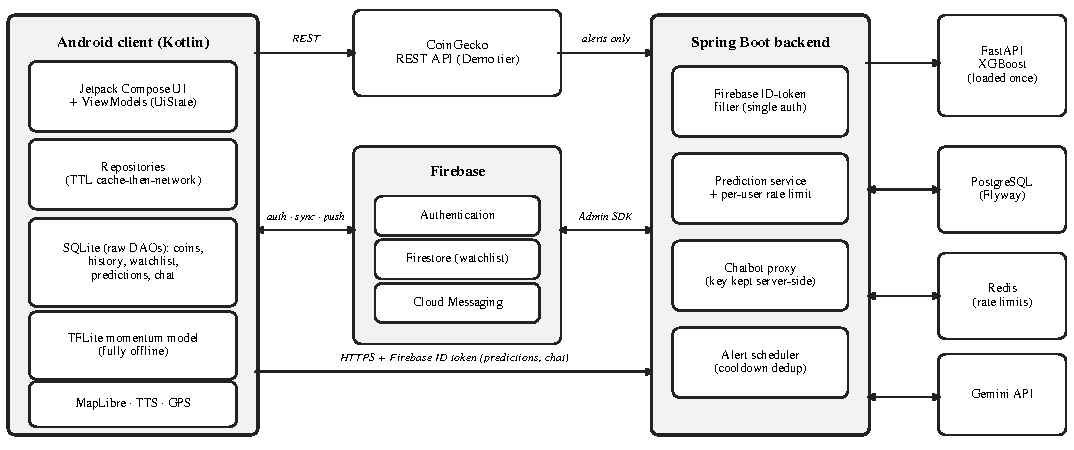
\includegraphics[width=\textwidth]{figs/fig_architecture.pdf}
\caption{System architecture. Market data comes directly from CoinGecko; predictions and chat go through the Spring Boot backend, which checks a Firebase ID token on every request. Dashed arrows are server-side calls used by the alert scheduler.}
\label{fig:architecture}
\end{figure*}

\begin{figure*}[t]
\centering
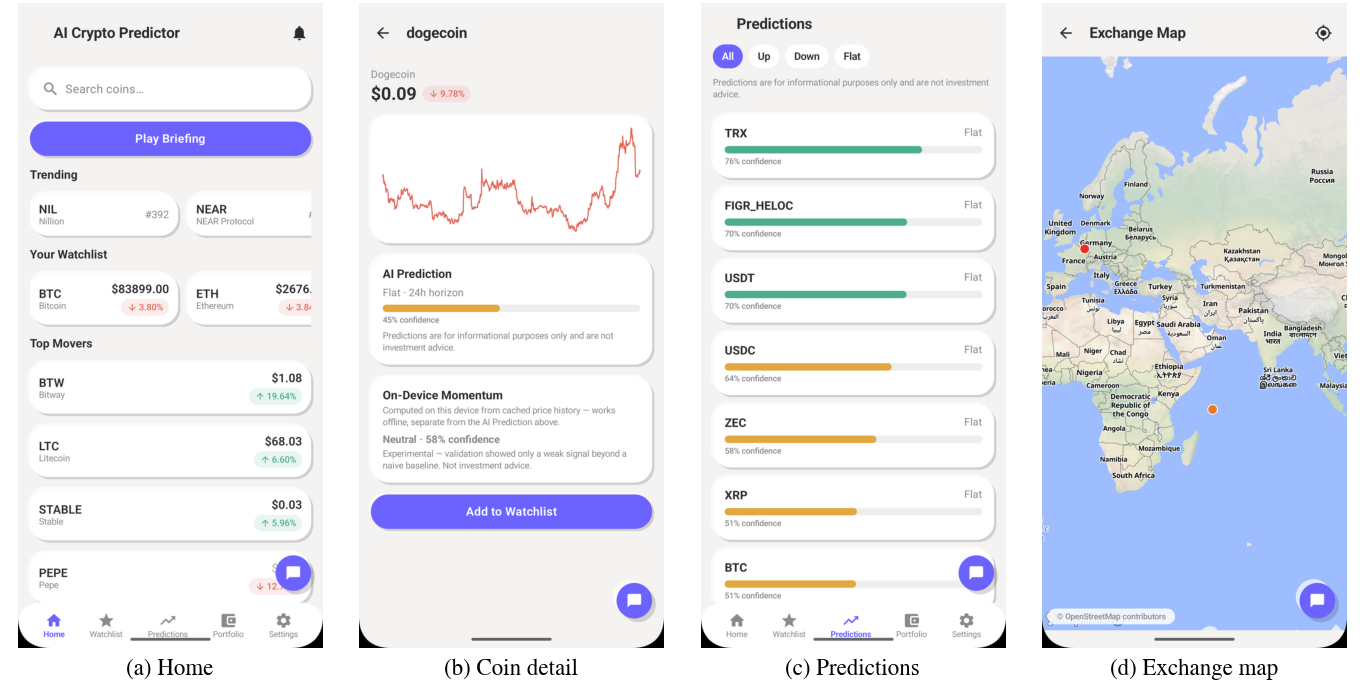
\includegraphics[width=0.88\textwidth]{figs/fig_ui.png}
\caption{Application screens: (a) home, (b) coin detail with chart, server prediction, on-device signal, and disclaimer, (c) predictions list, (d) exchange map.}
\label{fig:ui}
\end{figure*}

\begin{table}[t]
\caption{Technology Stack}
\label{tab:stack}
\centering
\begin{tabular}{p{0.22\columnwidth}p{0.66\columnwidth}}
\toprule
\textbf{Layer} & \textbf{Technology}\\
\midrule
Client & Kotlin, Jetpack Compose, Navigation, Retrofit, kotlinx.serialization\\
Local storage & SQLite (raw SQLiteOpenHelper, one DAO per table)\\
Cloud & Firebase Authentication, Firestore, FCM, Crashlytics\\
Backend & Java, Spring Boot, Spring Security, PostgreSQL, Flyway, Redis\\
AI service & Python, FastAPI, XGBoost\\
On-device ML & TensorFlow Lite\\
Assistant & Gemini through a backend proxy\\
Maps / audio & MapLibre with OpenFreeMap tiles; Android TextToSpeech\\
Deployment & Docker, Docker Compose, Nginx\\
\bottomrule
\end{tabular}
\end{table}

\textbf{Storage and sync.} The app keeps eight SQLite tables (watchlist, searches, settings, predictions, chat, notifications, coins, price history), each with its own DAO class. Firebase Authentication handles identity, Firestore holds each user's watchlist keyed by CoinGecko coin identifier, and Firebase Cloud Messaging (FCM) delivers alerts. Sync is last-write-wins using server timestamps, so differences between device clocks cannot corrupt the merge.

\textbf{Backend.} A request filter verifies each Firebase ID token with the Admin SDK, so there is one authentication authority and no separate app tokens. PostgreSQL (with Flyway migrations) stores a per-coin prediction cache and an alert cooldown table. Redis enforces per-user limits of 20 chatbot and 60 prediction requests per hour. The Python service is the only place with feature or model code, so a model can be retrained or replaced without touching Java or Kotlin.

\section{Methodology}

\subsection{Data}
The app uses the CoinGecko Demo API \cite{coingecko} (\texttt{/coins/markets}, \texttt{/coins/\{id\}}, \texttt{/market\_chart}, \texttt{/search}, \texttt{/search/trending}). The \texttt{top\_gainers\_losers} endpoint returned HTTP 401 on this tier, so the app ranks gainers and losers itself from the markets list. Coins are keyed by CoinGecko identifier (e.g., \texttt{bitcoin}), never by ticker symbol, because symbols are not unique.

Training data is one year (roughly August 2025 to August 2026) of daily prices and volumes for twelve large coins: Bitcoin, Ethereum, Solana, BNB, XRP, Cardano, Dogecoin, Polkadot, Chainlink, Litecoin, Avalanche, and TRON. After dropping a 40-day indicator warm-up and the last unlabeled day, each coin gives 325 samples, so 3,900 in total. Indicator warm-up is the only source of missing values, and a check confirms none remain. We apply no scaling (trees do not need it) and no outlier removal (large moves are what we want to model). Bitcoin's series is matched to each coin by nearest timestamp, since exact matching silently drops the newest point. The prediction endpoint rejects histories shorter than 41 points.

\subsection{Features and Labels}
Features are pure functions of a price and volume series. With closing price $P_t$, the daily return is $r_t=(P_t-P_{t-1})/P_{t-1}$, and the relative strength index \cite{wilder1978} is
\begin{equation}
RSI = 100 - \frac{100}{1+RS},
\end{equation}
where $RS$ is the 14-day average gain divided by the 14-day average loss. Crypto-specific features capture how strongly a coin follows Bitcoin. Over a trailing 30-day window, with $r^{B}_t$ the Bitcoin return,
\begin{equation}
\rho_t=\mathrm{corr}(r,r^{B}),\qquad
\beta_t=\frac{\mathrm{cov}(r,r^{B})}{\mathrm{var}(r^{B})}.
\end{equation}
Table~\ref{tab:features} lists all twenty numeric features; the coin identifier is added as a categorical feature.

\begin{table}[t]
\caption{Feature Set (20 Numeric Features Plus Coin Identifier)}
\label{tab:features}
\centering
\begin{tabular}{p{0.23\columnwidth}p{0.66\columnwidth}}
\toprule
\textbf{Family} & \textbf{Features}\\
\midrule
Trend & SMA (7, 14, 30 d); EMA (12, 26 d)\\
Momentum & RSI (14 d); MACD line, signal, histogram; ROC (1, 7 d)\\
Volatility & Bollinger upper, lower, bandwidth; return std.\ (7, 14 d)\\
Volume & 14-day volume ratio\\
Bitcoin-relative & BTC 24 h return; 30-day correlation and beta\\
\bottomrule
\end{tabular}
\end{table}

The label is the next day's move, with threshold $\tau=1.5\%$:
\begin{equation}
y_t=\begin{cases}
\mathrm{UP}, & (P_{t+1}-P_t)/P_t>\tau,\\
\mathrm{DOWN}, & (P_{t+1}-P_t)/P_t<-\tau,\\
\mathrm{FLAT}, & \text{otherwise.}
\end{cases}
\end{equation}
We compared four thresholds. At 1.0\% routine volatility counts as direction; at 2.0\% and 2.5\% FLAT grows to 58\% and 67\% of samples, rewarding a trivial always-FLAT guess. At 1.5\% the classes are 22.4\% UP, 29.5\% DOWN, and 48.1\% FLAT.

\subsection{Models}
\textbf{Server model.} An XGBoost classifier uses 300 trees of depth 4, learning rate 0.05, 0.8 row and column subsampling, native handling of the coin identifier, and seed 42. It minimizes a regularized softmax cross-entropy \cite{chen2016}. No class weighting or calibration is used: the reported confidence is the raw top class probability, and the target price is the current price moved by $\pm\tau$ for a directional output. The model loads once at service startup.

\textbf{Split with purge gap.} Shuffling price history leaks the future into training \cite{bergmeir2012,lopez2018}. All twelve coins share one calendar, so we use a single cutoff $T_s$ at the 80th percentile of timestamps (16 June 2026). Because each label looks one day ahead, a purge gap $\Delta=2$ days separates the sets:
\begin{equation}
\begin{aligned}
D_{\mathrm{train}}&=\{(x_t,y_t):t+\Delta<T_s\},\\
D_{\mathrm{val}}&=\{(x_t,y_t):t\geq T_s\}.
\end{aligned}
\label{eq:split}
\end{equation}
This gives 3,096 training and 780 validation samples.

\textbf{On-device model.} A bundled TensorFlow Lite model runs fully offline. Its inputs are only the 1-, 3-, and 7-day percentage returns, each a single subtraction and division, so the app can compute them without any feature-engineering code. The network has eight hidden ReLU units and a three-way softmax, is trained for 30 epochs on the same pooled data and purge rule (cutoff 9 June 2026; 3,408 training and 864 validation samples), and is quantized for size. It is shown beside, never instead of, the server prediction and is labeled experimental.

\subsection{Prediction Pipeline}
Figure~\ref{fig:pipeline} shows the path. The app already caches each coin's history, so it sends that history and Bitcoin's to the backend. As a result, neither the backend nor the AI service ever calls the market-data provider, which keeps one provider integration in the system. The backend authenticates the request, applies the rate limit, and reuses a cached prediction for 20 minutes before calling FastAPI. The app stores each result with separate generated and cached timestamps so stale entries are visible, and falls back to the cached value if a call fails. A disclaimer (``informational only, not investment advice'') appears on the detail card and on every row of the predictions list.

\begin{figure*}[t]
\centering
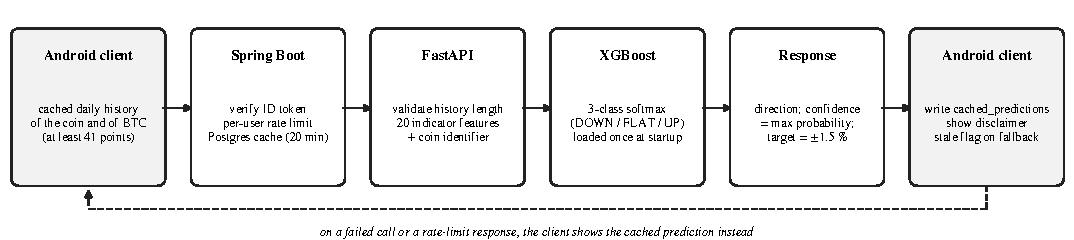
\includegraphics[width=\textwidth]{figs/fig_pipeline.pdf}
\caption{Prediction pipeline from cached history to a displayed prediction, including the cached-value fallback.}
\label{fig:pipeline}
\end{figure*}

\section{System Implementation}
\textbf{Market-data repository.} \texttt{CoinRepository} reads from SQLite first. A cached entry saved at time $t_c$ is served without a network call while
\begin{equation}
t_{\mathrm{now}}-t_c < TTL,
\end{equation}
where TTL is 60 s for the market list, 120 s for coin detail, 6 h for price history, and 5 min for trending coins. The same rule covers both the full list and filtered queries such as the watchlist. If the network fails, expired cache is shown with an \texttt{isStale} flag, so the screen says ``cached data'' instead of pretending to be current. Overlapping calls are merged with a mutex, and every catch block rethrows \texttt{CancellationException} first, so a cancelled request cannot overwrite newer data. Search is debounced by 300 ms. An empty search (HTTP 200) or unknown coin (404) shows an Empty state, while 429, 5xx, and timeouts show an error with a retry button. The Demo-tier API key is compiled into the app as a documented exception because it is low-privilege and easy to rotate; the chatbot key never is.

\textbf{Sync and backend.} On login, Firestore documents are merged into SQLite by server timestamp; later writes are pushed from a repository layer, a listener brings in changes from other devices, and Firestore's offline persistence queues edits made without a connection. Requests without a valid token get HTTP 401, and another user's resource returns 404 rather than 403 so its existence is not revealed.

\textbf{Chatbot, map, audio, and alerts.} The chatbot calls Gemini through the backend, so its key exists only in server configuration, and history is saved locally. The exchange map uses MapLibre with OpenFreeMap tiles (no API key) and joins exchange locations with live 24-hour volume from CoinGecko. A ``Locate me'' button takes one location fix (no continuous tracking), finds the nearest exchange with the haversine formula, and reads a one-sentence summary aloud with TextToSpeech, combining network, map, speech, and GPS. A scheduled server job sends an FCM alert when a watchlist coin moves at least 5\% in 24 hours or a cached prediction reaches 70\% confidence; both thresholds are configurable, a 60-minute cooldown prevents repeats, and the alert carries the coin identifier so a tap opens the right screen.

\textbf{Deployment.} The backend, AI service, PostgreSQL, Redis, and Nginx run as a five-service Docker Compose stack that builds on both ARM64 and AMD64. The release build uses R8, signing, Crashlytics, a privacy-policy screen, and the prediction disclaimer; debug-only tools are removed from it.

\section{Evaluation}

\subsection{Setup}
Both models are scored on a time-ordered hold-out as in~\eqref{eq:split}. Because classes are imbalanced, accuracy misleads: always predicting FLAT scores 0.60 accuracy yet finds no moves. We therefore use macro F1 (the mean of the three per-class F1 scores) with per-class precision $P_k$ and recall $R_k$:
\begin{equation}
\mathrm{Macro\text{-}F1}=\frac{1}{3}\sum_{k=1}^{3}\frac{2P_kR_k}{P_k+R_k}.
\end{equation}
Two baselines accompany the server model: \emph{majority class}, and \emph{persistence}, which assumes tomorrow repeats today's direction. The on-device model has its own majority baseline. We used Python 3.13, XGBoost 2.1.3, scikit-learn 1.5.2, pandas 2.2.3, and TensorFlow 2.21.0.

\subsection{System Verification}
Six automated tests cover the AI service's model loading (single load at startup, no reload per request, and a clear failure if the model file is missing), and all pass. The backend has further JUnit tests for alerts, controllers, and authentication. We also tested a debug build and a signed R8 release build on a Pixel~8 emulator (API~37) with the local Docker stack. Table~\ref{tab:verification} summarizes what was verified and how.

\begin{table}[t]
\caption{Verification Status}
\label{tab:verification}
\centering
\begin{tabular}{p{0.58\columnwidth}p{0.3\columnwidth}}
\toprule
\textbf{Behavior} & \textbf{Status}\\
\midrule
Debug and signed R8 release builds on emulator & Verified manually\\
Prediction endpoint returns real inference (HTTP 200) & Verified\\
Chatbot reply through backend proxy (Gemini) & Verified\\
Locate-me: success, denied, no-fix & Verified, simulated GPS\\
Docker Compose stack, end to end & Verified locally\\
Stale-cache display, rate-limit handling, no refetch within TTL & Implemented; code-reviewed and traced\\
\bottomrule
\end{tabular}
\end{table}

\section{Results and Discussion}
Table~\ref{tab:results} and Fig.~\ref{fig:results} give the results. XGBoost has the best macro F1 of the three server-side predictors (0.39, against 0.37 for persistence and 0.25 for the majority class). Its accuracy (0.56) is below the majority baseline's (0.60), which is expected: the majority baseline never detects a move, while the model does.

\begin{table*}[t]
\caption{Held-Out Results (Precision / Recall per Class)}
\label{tab:results}
\centering
\begin{tabular}{llcccccc}
\toprule
\textbf{Split} & \textbf{Model} & \textbf{Acc.} & \textbf{Macro F1} & \textbf{DOWN P/R} & \textbf{FLAT P/R} & \textbf{UP P/R}\\
\midrule
Server ($n{=}780$) & Majority class & 0.60 & 0.25 & 0.00 / 0.00 & 0.60 / 1.00 & 0.00 / 0.00\\
 & Persistence & 0.48 & 0.37 & 0.28 / 0.28 & 0.62 / 0.63 & 0.22 / 0.20\\
 & XGBoost (20 features + coin) & 0.56 & \textbf{0.39} & 0.35 / 0.21 & 0.66 / 0.82 & 0.21 / 0.14\\
\midrule
Device ($n{=}864$) & Majority class & 0.59 & 0.25 & 0.00 / 0.00 & 0.59 / 1.00 & 0.00 / 0.00\\
 & TFLite momentum (3 inputs) & 0.58 & \textbf{0.30} & 0.36 / 0.10 & 0.60 / 0.95 & 0.00 / 0.00\\
\bottomrule
\end{tabular}
\end{table*}

\begin{figure*}[t]
\centering
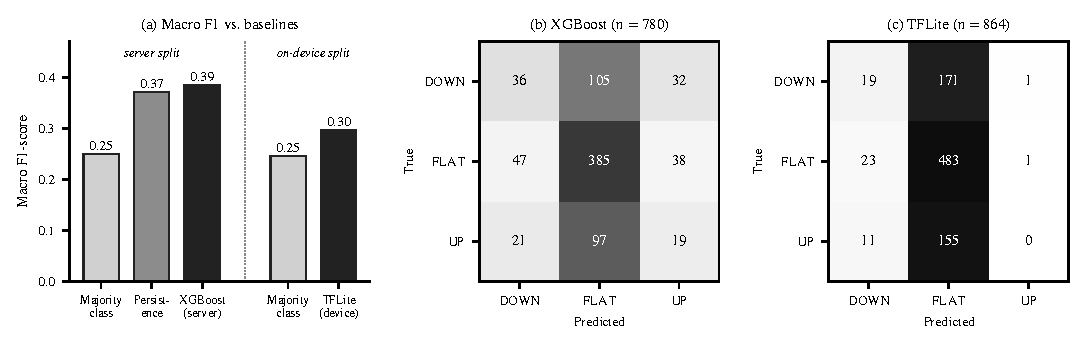
\includegraphics[width=\textwidth]{figs/fig_results.pdf}
\caption{(a) Macro F1 of each model against its baselines. (b), (c) Confusion matrices (counts; shading is row-normalized) for the server and on-device models.}
\label{fig:results}
\end{figure*}

A simple way to read the result is precision against each class's base rate. When the model predicts DOWN it is right 35\% of the time against a 22\% base rate (1.6 times better), and for UP 21\% against 18\% (1.2 times). So the model carries a small but real directional signal that the majority baseline lacks. This fits the low signal-to-noise ratio of return prediction \cite{gu2020} and the efficient-market view \cite{fama1970}, and it is why the app presents predictions as informational signals with explicit confidence, not as trading advice.

The on-device model, with only three inputs, beats its majority baseline (0.30 against 0.25) and finds some DOWN moves at 0.36 precision, but it does not detect UP moves. It therefore serves as a secondary offline hint, separate from the server prediction, which keeps the two signals independent and the app useful without a network.

Development also produced practical lessons. An endpoint that looked available in documentation was blocked on the free tier, and only live testing showed this. TTL caching applied to only the obvious call caused redundant requests for filtered queries. Catching a bare exception in cancellable coroutines let superseded requests update shared state until cancellation was rethrown. Finally, the ViewModel and UiState boundary let three successive data sources replace mock data without changing any screen.

\section{Limitations and Future Work}
Results come from one time-ordered split over a single year in which down days outnumbered up days; they are not a trading backtest and imply no profitability. The next model step is a walk-forward study with purged folds \cite{bergmeir2012,lopez2018}, adding LSTM and GRU models \cite{hochreiter1997,cho2014} behind the existing model interface, calibrated three-way probabilities, and later sentiment features \cite{bollen2011}.

On the systems side, the app calls CoinGecko directly through an interface built so a backend proxy can replace it and remove the client-held key. The portfolio screen currently uses sample data pending local persistence and sync, and the backend's symbol-keyed watchlist tables should be aligned with the client's coin-identifier keys before they are connected. Offline and rate-limit behavior will be tested on physical devices, followed by a user study.

\section{Conclusion}
AI Crypto Predictor couples a cache-tolerant Android client with a Spring Boot backend, a Python XGBoost service, an offline on-device model, a chatbot, a map, and alerts. Its design keeps all ML in one replaceable service, survives provider failures through TTL caching and stale fallback, uses one authentication authority and server-side secrets, and shows its uncertainty in the interface. Under leakage-controlled evaluation, the server model lifts macro F1 from 0.25 to 0.39 and the on-device model from 0.25 to 0.30. It is a complete platform on which stronger models and more rigorous evaluation can be built without redesigning the product.

\begin{thebibliography}{17}

\bibitem{fama1970}
E. F. Fama, ``Efficient capital markets: A review of theory and empirical work,'' \emph{J. Finance}, vol. 25, no. 2, pp. 383--417, May 1970, doi: 10.2307/2325486.

\bibitem{sezer2020}
O. B. Sezer, M. U. Gudelek, and A. M. Ozbayoglu, ``Financial time series forecasting with deep learning: A systematic literature review: 2005--2019,'' \emph{Appl. Soft Comput.}, vol. 90, Art. no. 106181, May 2020, doi: 10.1016/j.asoc.2020.106181.

\bibitem{hochreiter1997}
S. Hochreiter and J. Schmidhuber, ``Long short-term memory,'' \emph{Neural Comput.}, vol. 9, no. 8, pp. 1735--1780, Nov. 1997, doi: 10.1162/neco.1997.9.8.1735.

\bibitem{cho2014}
K. Cho \emph{et al.}, ``Learning phrase representations using RNN encoder-decoder for statistical machine translation,'' in \emph{Proc. Conf. Empirical Methods Natural Lang. Process. (EMNLP)}, Doha, Qatar, 2014, pp. 1724--1734, doi: 10.3115/v1/D14-1179.

\bibitem{chung2014}
J. Chung, C. Gulcehre, K. Cho, and Y. Bengio, ``Empirical evaluation of gated recurrent neural networks on sequence modeling,'' arXiv:1412.3555, 2014.

\bibitem{nelson2017}
D. M. Q. Nelson, A. C. M. Pereira, and R. A. de Oliveira, ``Stock market's price movement prediction with LSTM neural networks,'' in \emph{Proc. Int. Joint Conf. Neural Netw. (IJCNN)}, Anchorage, AK, USA, 2017, pp. 1419--1426, doi: 10.1109/IJCNN.2017.7966019.

\bibitem{fischer2018}
T. Fischer and C. Krauss, ``Deep learning with long short-term memory networks for financial market predictions,'' \emph{Eur. J. Oper. Res.}, vol. 270, no. 2, pp. 654--669, Oct. 2018, doi: 10.1016/j.ejor.2017.11.054.

\bibitem{mcnally2018}
S. McNally, J. Roche, and S. Caton, ``Predicting the price of Bitcoin using machine learning,'' in \emph{Proc. 26th Euromicro Int. Conf. Parallel, Distrib. Netw.-Based Process. (PDP)}, Cambridge, U.K., 2018, pp. 339--343, doi: 10.1109/PDP2018.2018.00060.

\bibitem{sebastiao2021}
H. Sebasti\~ao and P. Godinho, ``Forecasting and trading cryptocurrencies with machine learning under changing market conditions,'' \emph{Financ. Innov.}, vol. 7, Art. no. 3, 2021, doi: 10.1186/s40854-020-00217-x.

\bibitem{chen2016}
T. Chen and C. Guestrin, ``XGBoost: A scalable tree boosting system,'' in \emph{Proc. 22nd ACM SIGKDD Int. Conf. Knowl. Discovery Data Mining}, San Francisco, CA, USA, 2016, pp. 785--794, doi: 10.1145/2939672.2939785.

\bibitem{grinsztajn2022}
L. Grinsztajn, E. Oyallon, and G. Varoquaux, ``Why do tree-based models still outperform deep learning on typical tabular data?'' in \emph{Adv. Neural Inf. Process. Syst. (NeurIPS), Datasets Benchmarks Track}, 2022, arXiv:2207.08815.

\bibitem{gu2020}
S. Gu, B. Kelly, and D. Xiu, ``Empirical asset pricing via machine learning,'' \emph{Rev. Financ. Stud.}, vol. 33, no. 5, pp. 2223--2273, May 2020, doi: 10.1093/rfs/hhaa009.

\bibitem{bergmeir2012}
C. Bergmeir and J. M. Ben\'itez, ``On the use of cross-validation for time series predictor evaluation,'' \emph{Inf. Sci.}, vol. 191, pp. 192--213, May 2012, doi: 10.1016/j.ins.2011.12.028.

\bibitem{lopez2018}
M. L\'opez de Prado, \emph{Advances in Financial Machine Learning}. Hoboken, NJ, USA: Wiley, 2018.

\bibitem{coingecko}
CoinGecko, ``CoinGecko API documentation.'' [Online]. Available: \url{https://docs.coingecko.com}. Accessed: Sep. 23, 2026.

\bibitem{wilder1978}
J. W. Wilder Jr., \emph{New Concepts in Technical Trading Systems}. Greensboro, NC, USA: Trend Research, 1978.

\bibitem{bollen2011}
J. Bollen, H. Mao, and X. Zeng, ``Twitter mood predicts the stock market,'' \emph{J. Comput. Sci.}, vol. 2, no. 1, pp. 1--8, Mar. 2011, doi: 10.1016/j.jocs.2010.12.007.

\end{thebibliography}

\end{document}
